

\documentclass{article}
\usepackage[utf8]{inputenc}
\usepackage[utf8]{inputenc}
\usepackage[T1]{fontenc}
\usepackage[english]{babel}
\usepackage{fullpage}
\usepackage{color}
\usepackage[table]{xcolor}
\usepackage{listings}
 
\definecolor{darkWhite}{rgb}{0.94,0.94,0.94}
 
\lstset{
  aboveskip=3mm,
  belowskip=-2mm,
  backgroundcolor=\color{darkWhite},
  basicstyle=\footnotesize,
  breakatwhitespace=false,
  breaklines=true,
  captionpos=b,
  commentstyle=\color{red},
  deletekeywords={...},
  escapeinside={\%*}{*)},
  extendedchars=true,
  framexleftmargin=16pt,
  framextopmargin=3pt,
  framexbottommargin=6pt,
  frame=tb,
  keepspaces=true,
  keywordstyle=\color{blue},
  language=C,
  literate=
  {²}{{\textsuperscript{2}}}1
  {⁴}{{\textsuperscript{4}}}1
  {⁶}{{\textsuperscript{6}}}1
  {⁸}{{\textsuperscript{8}}}1
  {€}{{\euro{}}}1
  {é}{{\'e}}1
  {è}{{\`{e}}}1
  {ê}{{\^{e}}}1
  {ë}{{\¨{e}}}1
  {É}{{\'{E}}}1
  {Ê}{{\^{E}}}1
  {û}{{\^{u}}}1
  {ù}{{\`{u}}}1
  {â}{{\^{a}}}1
  {à}{{\`{a}}}1
  {á}{{\'{a}}}1
  {ã}{{\~{a}}}1
  {Á}{{\'{A}}}1
  {Â}{{\^{A}}}1
  {Ã}{{\~{A}}}1
  {ç}{{\c{c}}}1
  {Ç}{{\c{C}}}1
  {õ}{{\~{o}}}1
  {ó}{{\'{o}}}1
  {ô}{{\^{o}}}1
  {Õ}{{\~{O}}}1
  {Ó}{{\'{O}}}1
  {Ô}{{\^{O}}}1
  {î}{{\^{i}}}1
  {Î}{{\^{I}}}1
  {í}{{\'{i}}}1
  {Í}{{\~{Í}}}1,
  morekeywords={*,...},
  numbers=left,
  numbersep=10pt,
  numberstyle=\tiny\color{black},
  rulecolor=\color{black},
  showspaces=false,
  showstringspaces=false,
  showtabs=false,
  stepnumber=1,
  stringstyle=\color{gray},
  tabsize=4,
  title=\lstname,
}
\usepackage{graphicx}
\title{HAI804I – Codage et compression multimédia
}
\author{Fabien Caballero}

\begin{document}

\maketitle
    \tableofcontents

\newpage

\begin{figure}[h]
\centerline{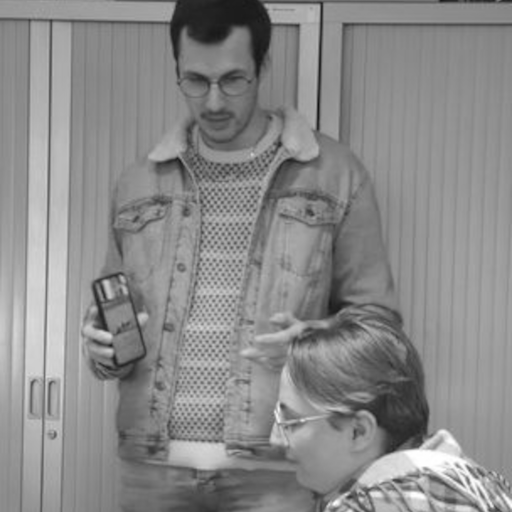
\includegraphics[scale=0.3]{./rendus/Maribault.png}}
\caption{Image d'origine utilisée tout le long du TP}
\end{figure}

\addcontentsline{toc}{section}{Introduction}
\section*{Introduction}
L'objectif de ce TP est de compresser une image avec un même algorithme mais avec et sans décorellation, qui consiste à prédire un pixel et garder seulement les erreurs de prédictions.
\\\\
\section{Espace des pixels: Compression d'Huffman sur l'image ppm originale}
Pour générer l'histogramme de l'image d'origine on utilise le programme créé dans un précédent TP.
Puis avec un programme, réalisant une compression de Huffman, on compresse l'image d'origine.
\begin{figure}[h]
\centerline{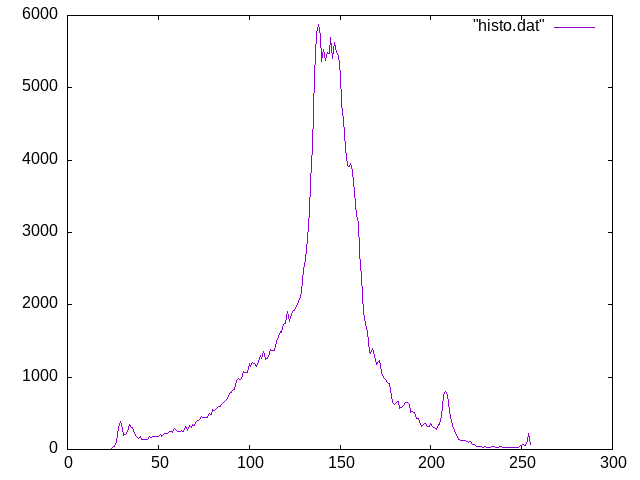
\includegraphics[scale=0.5]{./rendus/histo.png} }
\caption{histogramme de l'image d'origine}
\end{figure}
En compressant on obtient un taux de compression de t= taille de l'image d'origine / taille de l'image compressée

=> 262.2/228.2 =1.1489

\newpage
\section{Dans l'espace de prédiction}

\subsection{prédiction par précédent}
Pour générer la carte d'erreur pour chaque pixel on fait la différence entre la valeur prédite et la valeur réelle, dans ce partie la prédiction est la valeur du précédent pixel.
Afin de ne pas avoir de valeurs négatives on ajoute 128 àla valeur obtenue on a donc une image en niveau de gris.
\begin{figure}[h]
\centerline{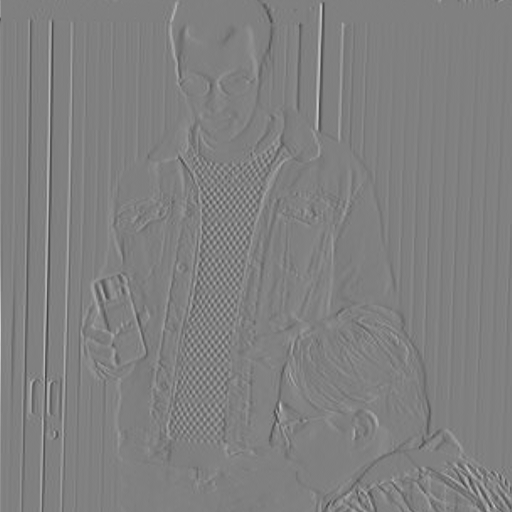
\includegraphics[scale=0.7]{./rendus/MaribaultErreurPredPrec.png} }
\caption{carte des différences}
\end{figure}

On réalise l'histogramme de cette image obtenue.

\begin{figure}[h]
\centerline{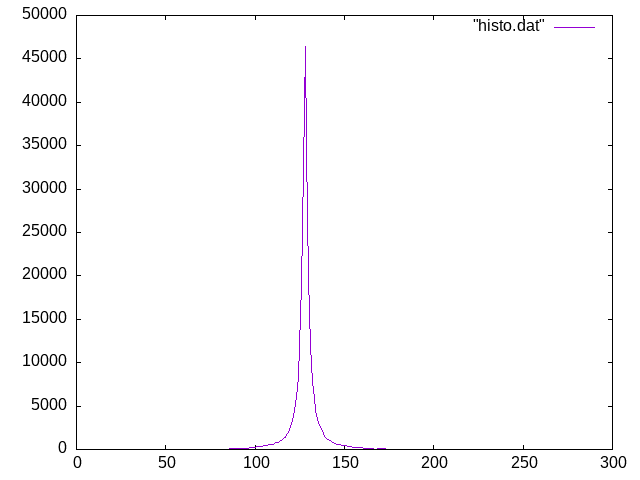
\includegraphics[scale=0.7]{./rendus/histoPredPrec.png} }
\caption{carte des différences}
\end{figure}

Taux de compression: taille de l'image d'origine / taille de l'image compressée

=> 262.2/146.6 =1.7885

\newpage
\subsection{prédiction avec (A+B)/2}
On fait exactement pareil avec cette fois-ci, on prend pour la prédiction de notre pixel la moyenne entre le pixel d'au dessus et du pixel à gauche du pixel courant.
\begin{figure}[h]
\centerline{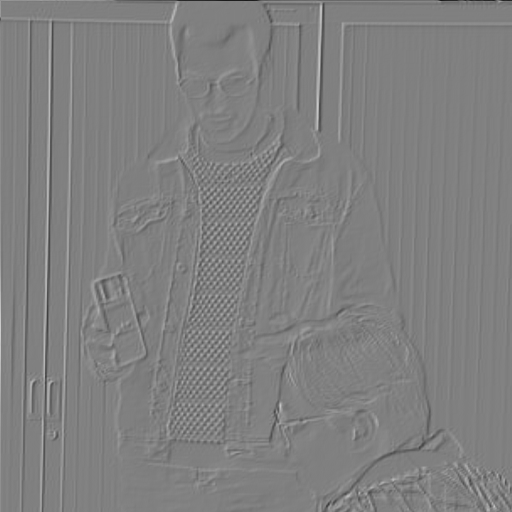
\includegraphics[scale=0.7]{./rendus/MaribaultErreurPredAplusBsur2.png} }
\caption{carte des différences}
\end{figure}

On remarque que le pic de l'histogramme est moins haut cela signifie que la compression sera moins efficace.
\begin{figure}[h]
\centerline{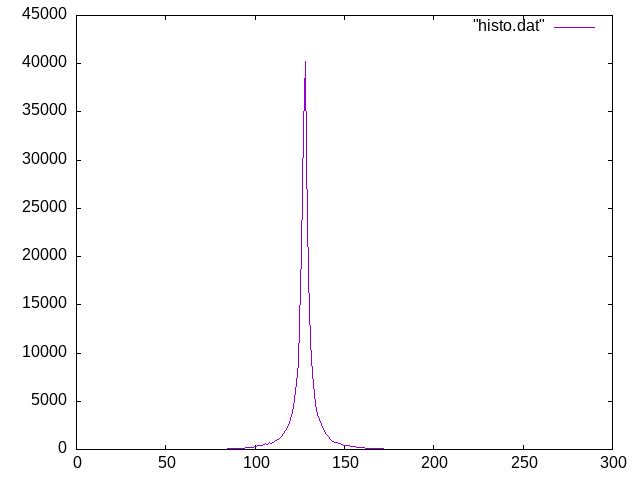
\includegraphics[scale=0.7]{./rendus/histoAplusBsur2.png} }
\caption{carte des différences}
\end{figure}

Taux de compression: taille de l'image d'origine / taille de l'image compressée

=> 262.2/151.8 =1.7272

On remarque en effet que le taux de compression est inférieur à celui d'un espace prédiction avec le précédent.

\addcontentsline{toc}{section}{Conclusion}
\section*{Conclusion}
On conclu que l'utilisation d'une image d'erreurs de prédictions est plus efficace lors d'une compression par rapport à une simple compression de l'image originale.
Utiliser différentes méthodes prédictions permet d'avoir de meilleurs taux de compression.
L'utilisation d'une carte d'erreur de prédictions permet de gagner permet de gagner 0,5 sur le taux de compression et une utilisation différente de prédictions permet de gagner un taux de compression de l'ordre de 0,1.

Une autre possibilité et d'utiliser DPCM afin d'obtenir un meilleur taux de compression.



\end{document}